\documentclass[]{achemso}

\usepackage{amsmath}        % Equation editing using flags of \begin{align} and \end{align}
\usepackage{graphicx}       % Display figures using \includegraphics
\graphicspath{{figures/}}   % Location for figures relative to .tex file path
\usepackage{etoolbox}       % Make the bibliograph unjustified (to work around hbox errors)
\apptocmd{\thebibliography}{\raggedright}{}{}
\usepackage{glossaries}     % Enable the \newacronym and \gls commands to reference terms

\newacronym{DFT}{DFT}{density functional theory}
\newacronym{FCC}{FCC}{face-centered cubic}
\newacronym{VASP}{VASP}{the Vienna Ab-initio Simulation Package}
\newacronym{GASpy}{GASpy}{the Generalized Adsorption Simulator for Python}
\newacronym{rPBE}{rPBE}{revised Perdew-Burke-Ernzerhof}
\newacronym{ASE}{ASE}{the Atomic Simulation Environment}


%\usepackage{booktabs}       % Use table things like \toprule or \bottomrule
%\usepackage[table]{xcolor}  % Lets us use \rowcolors to make alternate table shading
%\usepackage{makecell}       % Allow the use of the \makecell command that lets linebreaks in table cells
%\usepackage{pdflscape}      % Enable the \begin{landscape} command

% chktex-file 36


%%%%%%%%%%%%%%%%%%%% Title/Abstract %%%%%%%%%%%%%%%%%%%%
\title{Uncertainty Benchmark (placeholder)}
\author{Kevin Tran}
\affiliation{Department of Chemical Engineering, Carnegie Mellon University, Pittsburgh, PA 15217}
\altaffiliation{These authors contributed equally to this work}
\author{Willie Neiswanger}
\affiliation{Machine Learning Department, Carnegie Mellon University, Pittsburgh, PA 15217}
\altaffiliation{These authors contributed equally to this work}
\author{Junwoong Yoon}
\affiliation{Department of Chemical Engineering, Carnegie Mellon University, Pittsburgh, PA 15217}
\author{Eric Xing}
\affiliation{Machine Learning Department, Carnegie Mellon University, Pittsburgh, PA 15217}
\author{Zachary W. Ulissi}
\affiliation{Department of Chemical Engineering, Carnegie Mellon University, Pittsburgh, PA 15217}
\email{zulissi@andrew.cmu.edu}

\begin{document}

%\setlength{\fboxrule}{0 pt}
%\begin{tocentry}
%    \includegraphics[width=\textwidth]{TOC/TOC.pdf}
%    This perspective discusses three common tools used in informatics research:
%    databases, surrogate modeling, and workflow managers. Although these tools are not
%    new, they are relatively new in the field of surface science and catalysis. We
%    discuss how these tools can augment and accelerate surface science research, and we
%    provide examples from both literature and our own work. We also provide our
%    perspective on when to use these tools and some best practices to follow when
%    creating them.
%\end{tocentry}

\begin{abstract}
    Abstract here.
\end{abstract}


%%%%%%%%%%%%%%%%%%%% Introduction %%%%%%%%%%%%%%%%%%%%

\section{Introduction}

\begin{enumerate}
    \item{ML/DS + catalysis}

    \item{Why uncertainty?}
        \begin{enumerate}
            \item{want confidence on DFT predictions themselves}
            \item{active routines}
        \end{enumerate}

    \item{Very quick overview of the paper (Figure~\ref{fig:overview})}
\end{enumerate}

\begin{figure}
    \centering
    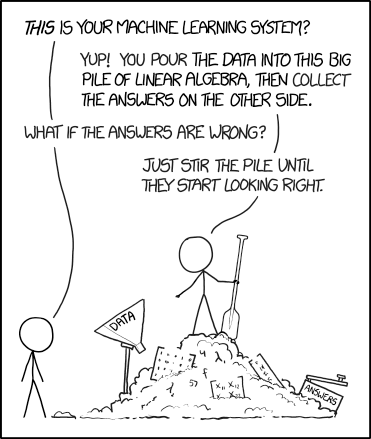
\includegraphics[width=0.5\textwidth]{placeholder.png}
    \caption{Placeholder for overview of the paper}\label{fig:overview}
\end{figure}


%%%%%%%%%%%%%%%%%%%% Methods %%%%%%%%%%%%%%%%%%%%

\section{Methods}

\subsection{Data handling}

All regressions in this paper were performed on a dataset of \gls{DFT} calculated adsorption energies created with \gls{GASpy}\cite{Tran2018, Tran2018a}.
These data included energies from 21,269 different H adsorption sites; 1,594 N sites; 18,437 CO sites; 2,515 O sites; and 3,464 OH sites; totaling in 47,279 data points.
\gls{GASpy} performed all \gls{DFT} calculations using \gls{VASP}\cite{Kresse1993, Kresse1994, Kresse1996, Kresse1996a} version 5.4 implemented in \gls{ASE}\cite{HjorthLarsen2017}.
The \gls{rPBE} functionals\cite{Hammer1999} were used along with \gls{VASP}'s pseudopotentials, and no spin magnetism or dispersion corrections were used.
Bulk relaxations were performed with a $10\times10\times10$ k-point grid and a 500 eV cutoff, and only isotropic relaxation were allowed during this bulk relaxation.
Slab relaxations were performed with k-point grids of $4\times4\times1$ and a 350 eV cutoff.
Slabs were replicated in the X/Y directions so that each cell was at least 4.5 \AA{} wide, which reduces adsorbate self-interaction.
Slabs were also replicated in the Z direction until they were at least 7 \AA{} thick, and at least 20 \AA{} of vacuum was included in between slabs.
The bottom layers of each slab were fixed and defined as those atoms more than 3 \AA{} from the top of the surface in the scaled Z direction.

To split the data into train/validate/test sets, we first enumerated all adsorption energies on monometallic slabs and added them to the training set manually. 
We did this because some of the regression methods in this paper use a featurization that contains our monometallic adsorption energy data\cite{Tran2018}, and so having the monometallic adsorption energies pre-allocated in the training set prevented any information leakage between the training set and validation/test sets.
After this allocation, we performed a 64/14/20 train/validate/test split that was stratified\cite{Thompson2012} by adsorbate.
We used the train/validate partitions to tune various hyperparameters manually.
To create the results shown in this paper, we combined the training and validation partitions into a single training set and reported models' performances on the held-out training set.

\begin{enumerate}
    \item{Modeling}
        \begin{enumerate}
            \item{CGCNN}
            \item{CGCNN Ensemble}
            \item{GP}
            \item{GP with CGCNN}
            \item{With other kernels too}
            \item{Penultimate-Fed GP}
            \item{Bayesian CGCNN with prior on weights at some layer}
            \item{Supervised error prediction (delta CGCNN)}
            \item{Dropout CGCNN}
        \end{enumerate}
    \item{Assessment}
        \begin{enumerate}
            \item{accuracy}
            \item{calibration}
            \item{sharpness}
        \end{enumerate}
\end{enumerate}


%%%%%%%%%%%%%%%%%%%% Results %%%%%%%%%%%%%%%%%%%%

\section{Results}

\begin{enumerate}
    \item{Table/figure of accuracies: MSE, MAE, R2, [willie get list]}
    \item{Plots:}
        \begin{enumerate}
            \item{Parity plots}
            \item{Calibration/sharpness plots}
            \item{Sharpness values per method}
        \end{enumerate}
    \item{Blocking results?}
    \item{Cost of computing each method (if it’s there)}
    \item{Human overhead and difficulty}
\end{enumerate}


%%%%%%%%%%%%%%%%%%%% Conclusions %%%%%%%%%%%%%%%%%%%%

\section{Conclusions}

Observations about relative accuracies, calibrations, sharpnesses, overhead


%%%%%%%%%%%%%%%%%%%% Misc %%%%%%%%%%%%%%%%%%%%

\section*{Code availability} Visit \texttt{https://github.com/ulissigroup/uncertainty\_benchmarking} for the code used to create the results discussed in this paper.
The code dependencies are listed inside the repository.

\section*{Author information} Corresponding author email:  zulissi@andrew.cmu.edu.
The authors declare no competing financial interest.

\section*{Acknowledgements} This research used resources of the National Energy Research Scientific Computing Center, a DOE Office of Science User Facility supported by the Office of Science of the U.S. Department of Energy under Contract No. DE-AC02-05CH11231. % chktex 8
% TODO add credit to NESAP
% TODO add credit to Willie's cluster


%%%%%%%%%%%%%%%%%%%% Bibliography %%%%%%%%%%%%%%%%%%%%

\clearpage
\bibliography{uncertainty_benchmarking}

\end{document}
